\documentclass{article}

% \usepackage{showframe}
% \usepackage[export]{adjustbox}
% \usepackage[a4paper, vmargin=1in]{geometry}
\usepackage{graphicx}
\usepackage{polski}
\usepackage{indentfirst}
\usepackage{fancyhdr}
\usepackage{float}
\usepackage{hyperref}
\usepackage{listings}

\lstset{basicstyle={\footnotesize\ttfamily}}

\pagestyle{fancy}
\fancyhf{}

\lhead{Architektura Komputerów 2}
\rhead{\thepage}

\begin{document}

% strona tytułowa
\begin{titlepage}
	\clearpage
	\thispagestyle{empty}
	\pagenumbering{gobble}
    \centering
    
	{\LARGE Architektura Komputerów 2 \par}
	
	\vspace{1.5cm}
	
	{\huge\bfseries Liczby zdenormalizowane\par}
	
	\vspace{1.5cm}
	{\large czwartek nieparzysty, 18:55\par}

	\vspace{1cm}
    \parbox{0.4\linewidth}{
	    \centering
	    {\Large Michał \textsc{Sieroń}\par}
	    {\large 256 259\par}
	}
    \hfill
    \parbox{0.4\linewidth}{
	    \centering
	    {\Large Paweł \textsc{Różański}\par}
	    {\large 252 772\par}
	}

	\vspace{1.5cm}
	{\large prowadzący\par}
	{\large dr inż. Piotr \textsc{Patronik}\par}
    
	\vfill

	{\large Informatyka Techniczna, Wydział Elektroniki\par}
	\vspace{0.5cm}
	{\large \today\par}
	\clearpage
	\pagenumbering{arabic}
\end{titlepage}

\tableofcontents
\newpage

\section{Wstęp}
Zadanie projektowe polegało na analizie zawartości artykułu i implementacji przedstawionych układów w języku \emph{Verilog}.
Z powodu ograniczonego czasu na wykonanie projektu możliwe było zaimplemenetowanie jedynie układów \emph{A1} oraz \emph{M} przedstawionych w artykule \cite{art:old}.

Następnie zaimplementowano odpowiadajace im układy zgodne ze standardem \emph{IEEE-754} \cite{art:ieee754} \cite{pdf:ieee754}.
Dokonano również porównania błędów wynikajacych z~użycia danej reprezentacji liczby zmiennoprzecinkowej. 


\section{Opis koncepcji zapisu i formatu}
Koncepcja formatu liczb zmiennoporzecinkowych, zaproponowanego w artykule \cite{art:old} wzięła się z~obserwacji, że standard \emph{IEEE-754} nie został stworzony z myślą o systemach wbudowanych.
Eliminacja logiki normalizującej powinna obniżyć koszt produkcji układu, a wpływ na precyzję obliczeń nie powinien mieć znaczenia w docelowych zastosowaniach.
Normalizacja liczby jest sktukiem używania ukrytej jedynki w liczbach znormalizowanych.
Sprawia to, że pojawia się wyjątek, który trzeba obsłużyć w sprzęcie.
Proponowany format pozbywa się ukrytej jedynki, kosztem jednego z bitów mantysy.
Konsekwencją tego jest zmniejszona precyzja liczb.


\section{Opis metody}
Wszystkie układy zostały zaimplementowane w języku opisu sprzętu \emph{Verilog}.
Jednak druga część projektu, która je ze sobą łączy i porównuje z wartością referencyjną, została napisana w języku \emph{Python}.
Dla zadanej ilości przypadków testowych generowaliśmy tyle samo par liczb typu \texttt{float}.
W języku \emph{Python}, typ \texttt{float} odpowiada liczbie zmiennoprzecinkowej o podwójnej precyzji.
Wobec tego konieczne było przekonwertowanie wygenerowanych liczb na liczbę zmiennoprzecinkową o pojedynczej precyzji.
W tym celu napisaliśmy funkcję \texttt{py2float} w języku \emph{C}, która zamienia wartość typu \texttt{double} na \texttt{float}.
Tak otrzymane wartości były następnie zamieniane na ich szesnastkową reprezentację.
W tym celu musieliśmy uprzednio otrzymać bajtową reprezentację danej liczby, która z~kolei była zamieniana na liczbę typu \texttt{int}, z której w końcu mogliśmy otrzymać reprezentację w systemie szesnastkowym.

Konwersję z liczby znormalizowanej na zdenormalizowaną zaimplementowaliśmy w tym samym skrypcie.
W ten sam sposób co wcześniej, otrzymywaliśmy zapis szesnastkowy liczby lecz denormalizacja liczby wymaga operacji bitowych.
Przez fakt użycia \emph{Pythona} konieczne było do tego zamienienie liczby na listę bitów (w tym przypadku liczb całkowitych typu \texttt{int} o wartościach 0 lub 1).
Tak otrzymana lista była następnie odpowiednio dzielona na części znaku, wykładnika i mantysy.
Mantysa była przesuwana o jedną pozycję w prawo, a wykładnik zwiększany o jeden.
Tak zmodyfikowaną reprezentację bitową zamienialiśmy z~powrotem na zapis szesnastkowy.

Wykorzystując wygenerowane pary liczb tworzyliśmy pliki \emph{Veriloga} wykorzystujące napisane przez nas moduły opisane w sekcji \ref{sec:implementacja}.
Utworzone pliki były następnie uruchamiane, a wyniki zapisywane w pliku \emph{csv} do dalszego przetwarzania.


\section{Opis implementacji}\label{sec:implementacja}

\subsection{Układy dodawania}
Implementacja układu dodawania liczb zmiennoprzecinkowych została wykonana na podstawie opisu oraz 
modelu układu z artykułu \cite{art:old}.
Według nazewnictwa z artykułu układ dodawania, który odwzorowaliśmy, to \emph{A1}. 
Jest to najprostsza wersja dodawania dwóch liczb zdenormalizowanych.

Implementację układu zaczęliśmy od dokładnego przeczytania opisu przedstawionego w~artykule, a następnie stworzeniu podstawowych bloków do obliczeń zawartych na diagramie \ref{fig:diagram_add_denorm}.

% schemat dodawania zdenormalizowanego
\begin{figure}[H]
	\centering
	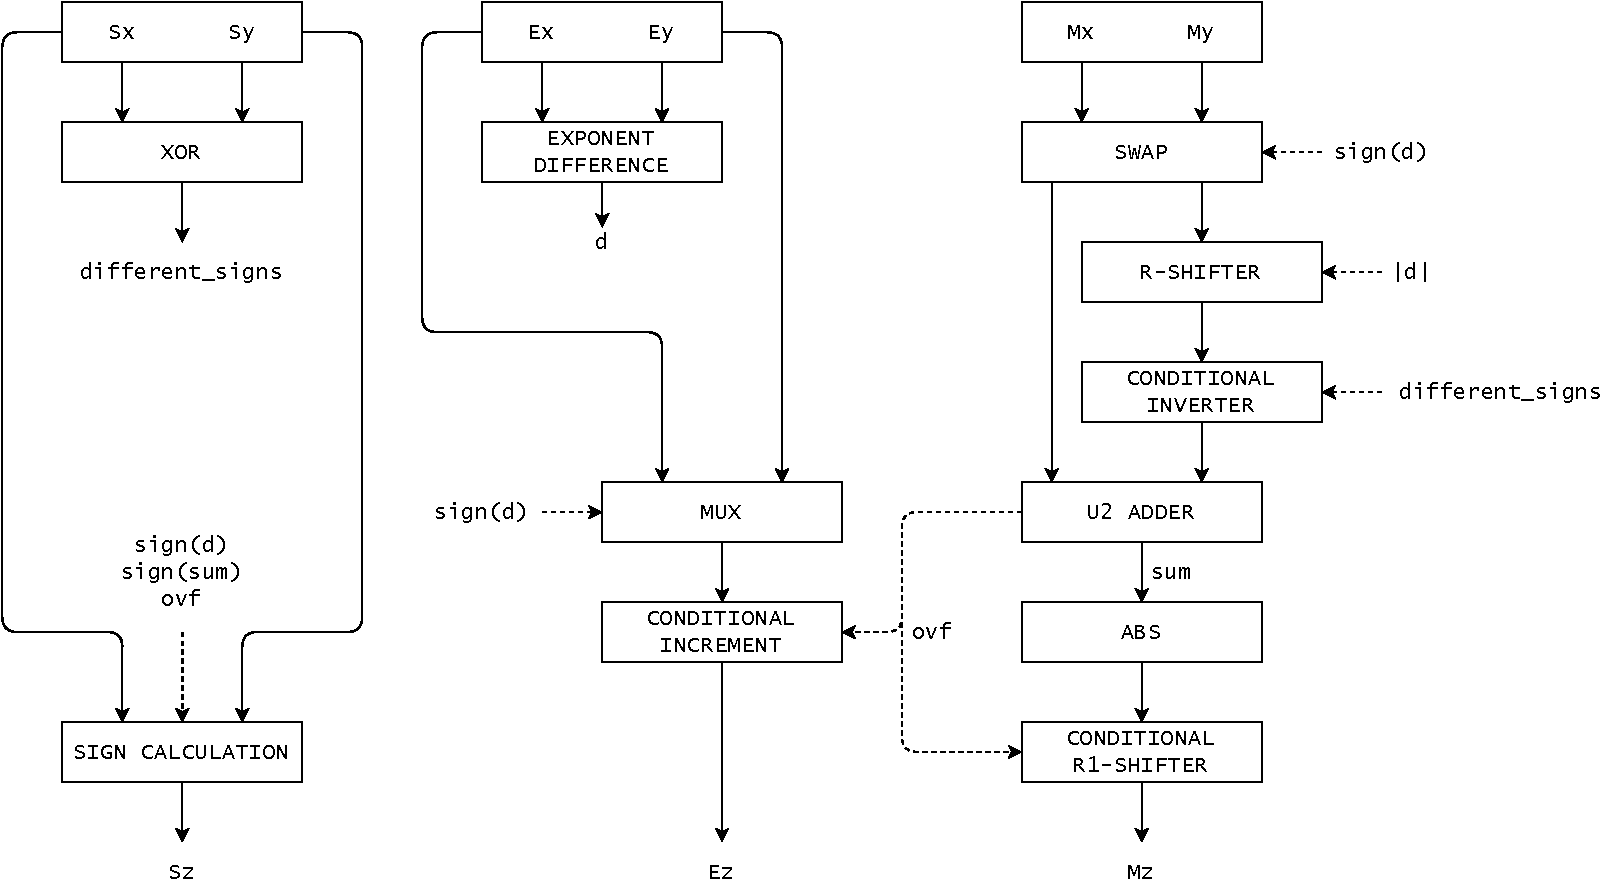
\includegraphics[width=\textwidth]{figures/diagram_add_denorm.pdf}
	\caption{Schemat układu dodawania - zdenormalizowane}
	\label{fig:diagram_add_denorm}
\end{figure}

Na początku układ oblicza różnicę wykładników, żeby następnie wyrównać drugą z nich do tej samej wartości wykładnika.
Liczba z mniejszym wykładnikiem jest przesuwana w prawo o ilość bitów równą wartości różnicy wykładników.
Jeżeli liczby mają różne znaki, to wyrównywana liczba jest dodatkowo negowana.
Umożliwia to sumowanie mantys w U2 wykorzystując obliczony wcześniej bit \texttt{different\_signs} jako przeniesienie wejściowe.
Wewnątrz sumatora wykrywane jest przepełnienie i po obliczeniu wartości bezwzględnej wyniku, wykorzystywane do ewentualnego przesunięcia go w prawo o jeden bit.
W~takim przypadku zwiększany jest też wykładnik wyjściowy.
Wyznaczenie znaku w~przypadku liczb zdenormalizowanych nie jest łatwe.
Wynika to z faktu, że nawet gdy wykładnik jednej z liczb jest większy od drugiej, to różnica w~mantysach może być jeszcze większa.
Wobec tego, konieczne jest wykorzystanie znaków różnicy wykładników, sumy mantys oraz bitu \texttt{ovf} informującym o~przepełnieniu.

Zaimplementowany przez nas układ dodawania liczb znormalizowanych oparty jest o wersję zdenormalizowaną.
Różnice zaznaczyliśmy na rysunku \ref{fig:diagram_add_ieee754} na zielono.

% schemat dodawania IEEE-754
\begin{figure}[H]
	\centering
	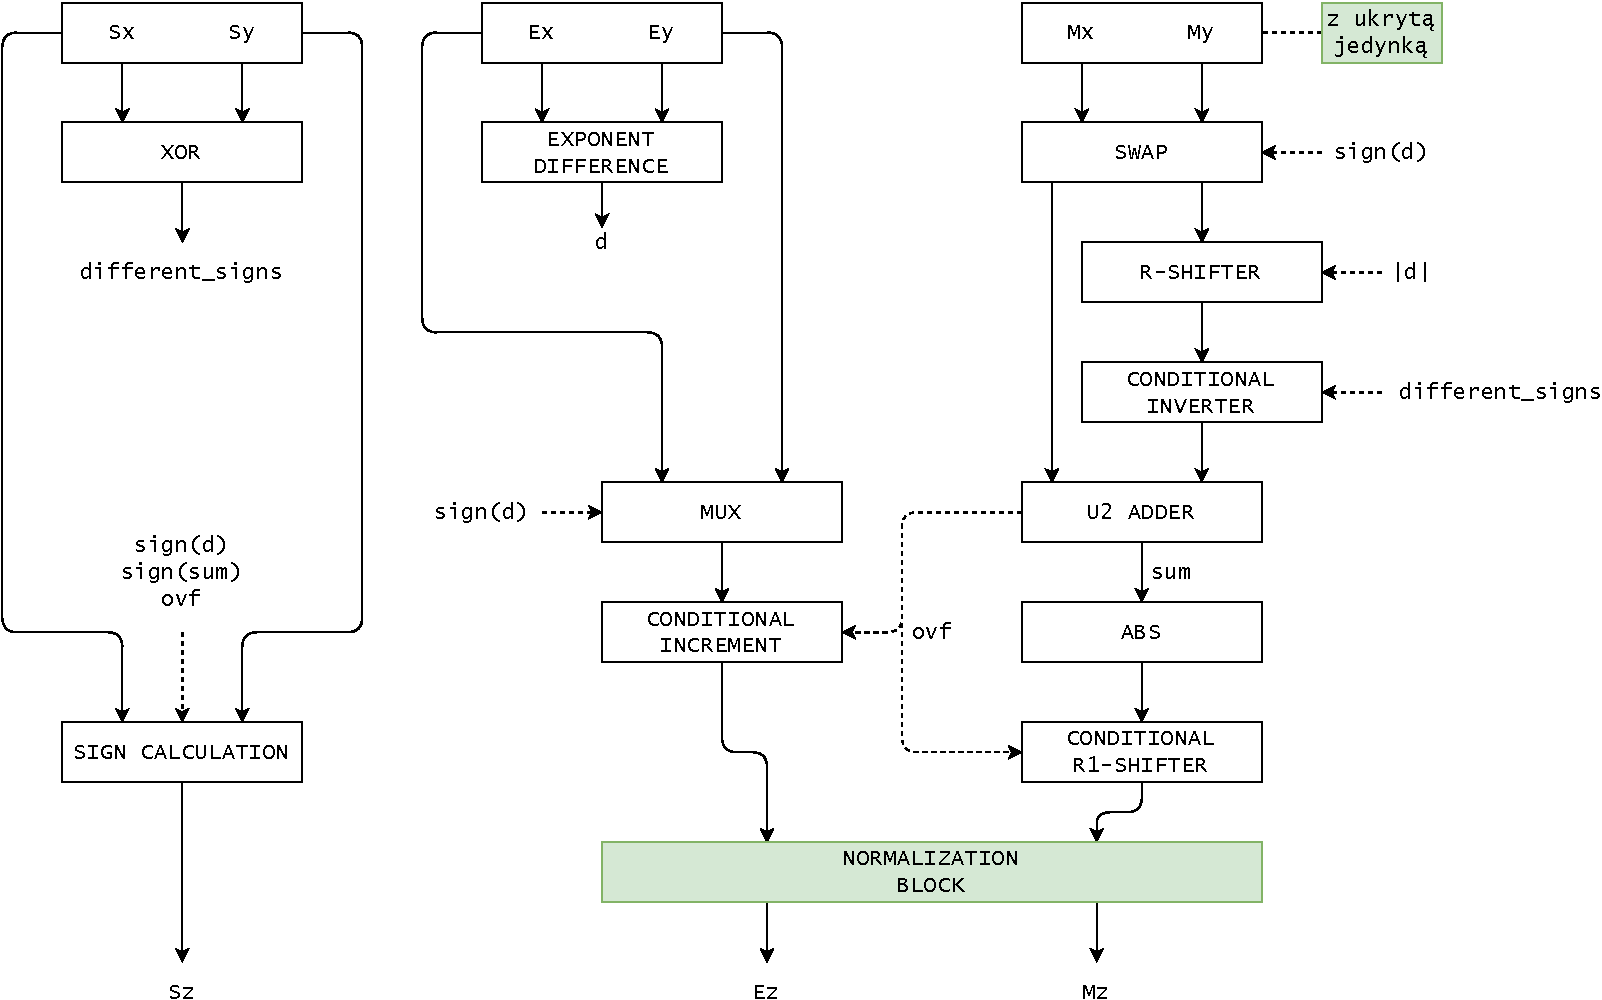
\includegraphics[width=\textwidth]{figures/diagram_add_ieee754.pdf}
	\caption{Schemat układu dodawania - \emph{IEEE-754}}
	\label{fig:diagram_add_ieee754}
\end{figure}

% napisać o znaku
Pierwszą zmianą jest warunkowe dodanie ukrytej jedynki.
Drugą zaznaczoną zmianą jest blok normalizacyjny.
Mantysa jest przesuwana w lewo dopóki na pozycji ukrytego bitu nie pojawi się 1.
Natomiast inną zmianą, która nie jest uwzględniona na schemacie, jest szerokość bitowa sumy mantys.
W wersji liczb znormalizowanych ma ona 48 bitów.

\subsection{Układy mnożenia}

Kolejnym układem, który zaimplementowaliśmy, był układ mnożący, który podobnie jak układ dodawania pochodzi z artykułu \cite{art:old}.
Autorzy nadali mu nazwę \emph{M}.
Jest to pierwsza wersja zaproponowanej przez autorów implementacji układu mnożenia liczb zdenormalizowanych.

% schemat mnożenia zdenormalizowanego
\begin{figure}[H]
	\centering
	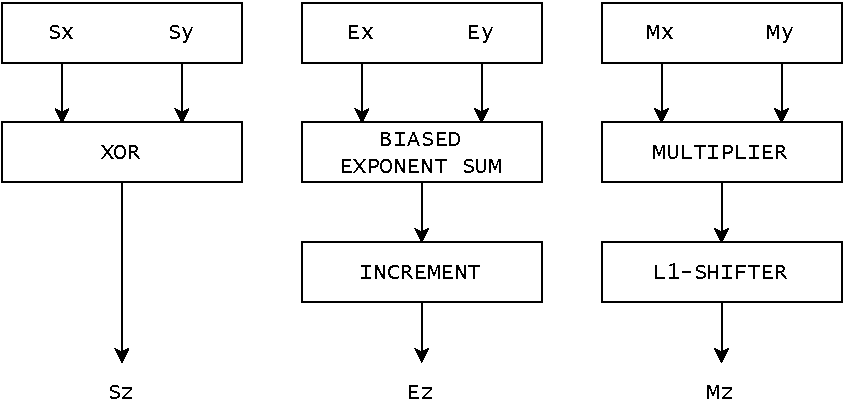
\includegraphics[width=\textwidth]{figures/diagram_mul_denorm.pdf}
	\caption{Schemat układu mnożenia - zdenormalizowane}
	\label{fig:diagram_mul_denorm}
\end{figure}

W przeciwieństwie do sumatora, wyznaczenie znaku jest prostą operacją \texttt{XOR}.
Wykładnik jest sumą wykładników wejściowych z odjętym obciążeniem.
Autorzy przyjęli założenie, że operacja mnożenia mantys, zawsze zakończy się przepełnieniem.
Wobec tego wykładnik wyjściowy jest zawsze zwiększany o jeden, a~mantysa przesuwana w prawo.
W przypadku braku wystąpienia przepełnienia, tracony jest jeden bit precyzji.

Zmiany względem układu mnożącego liczby zgodne ze standardem \emph{IEEE-754} są w tym przypadku niewielkie.

% schemat mnozenia IEEE-754
\begin{figure}[H]
	\centering
	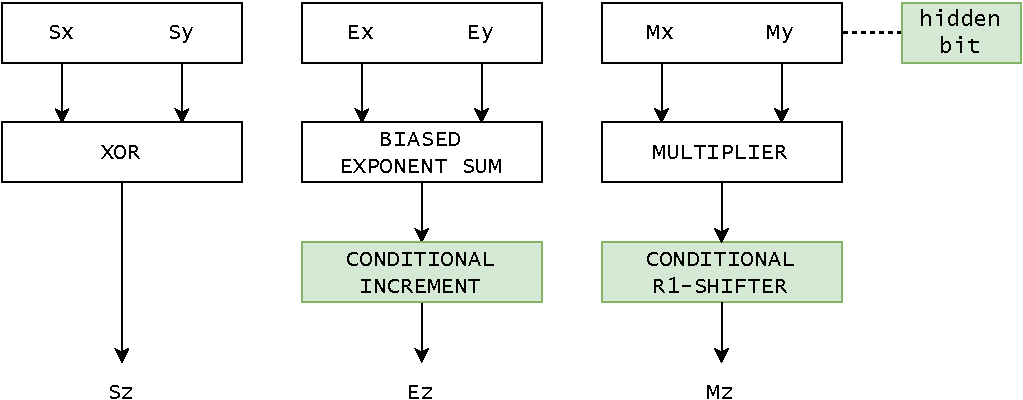
\includegraphics[width=\textwidth]{figures/diagram_mul_ieee754.pdf}
	\caption{Schemat układu mnożenia - \emph{IEEE-754}}
	\label{fig:diagram_mul_ieee754}
\end{figure}

Ponieważ wynik mnożenia dwóch licz znormalizowanych gwarantuje pojawienie się jedynki na jednym z dwóch najstarszych bitów wyniku, normalizacja sprowadza się do warunkowego przesunięcia w prawo w zależności od wystąpienia przepełnienia.


\section{Narzędzia}
Do implementacji układów dodawania i mnożenia użyliśmy języka \emph{Verilog}.
W \emph{C} napisaliśmy funkcje konwertujące wartości typu \texttt{double} na \texttt{float} konieczne do porówania wyników.
\emph{Python} służył jako język, z którego wywoływane były wszystkie polecenia kompilujące wcześniej wspomniane funkcje w \emph{C}, generujące oraz uruchamiające pliki testowe \emph{Veriloga}.
Przy użyciu \emph{Pythona} obliczaliśmy również błędy obliczeniowe wynikające z formatu zdenormalizowanych liczb zmiennoprzecinkowych oraz wykresy je prezentujące.
Do tworzenia wykresów posłużyliśmy się biblioteką \emph{Matplotlib}.
Narzędzie \emph{Icarus Verilog} posłużyło nam do kompilacji i~uruchamiania modułów napisanych w języku \emph{Verilog}.
Natomiast do sprawdzenia poprawności wyników poszczególnych bloków i debugowania programu używaliśmy programu \emph{GTKWave}.
Do utworzenia diagramów została użyta aplikacja \url{diagrams.net}.
Całość kodu była tworzona w programie \emph{Visual Studio Code}.
Testowanie i uruchamianie miało miejsce w systemie Ubuntu na maszynie wirtualnej \emph{WSL 2}.


\section{Opis sposobu testowania}
Stworzone układy sumatora i mnożenia liczb zdenormalizowanych zostały przetestowane pod względem różnic pomiędzy wynikami w swoich odpowiednikach w implementacji \emph{IEEE-754}.
Testowanie rozpoczeliśmy od wygenerowania liczb pseudolosowych w zakresie, w którym zadbaliśmy o to, aby nie doszło do przepełnienia wykładnika.
Wygenerowana liczba utworzona została w języku \emph{Python}, więc była podwójnej precyzji.
Przy pomocy zaimplementowanej przez nas funkcji, zmieniliśmy ją na liczbę pojedynczej precyzji.

Kolejnym krokiem w testowaniu było wykonanie odpowiednich dodawań lub mnożeń w zależności od testowanych układów.
Program następnie startował symulator uruchamiający kolejne układy.
Pierwszym z nich był zaimplementowany przez nas układ działający na liczbach zdenormalizowanych.
Drugim był układ częściowo zgodny ze standardem \emph{IEEE-754}.
Do tego obliczaliśmy wynik operacji na liczbach podwójnej precyzji, którego używaliśmy jako wartości referencyjnej do porównywania wyników.
Tak otrzymane liczby były zapisywane do plików \emph{CSV}.

Testowanie przeprowadzilismy dla następujących ilości wyników 100, 1 000, 10 000, 100 000, 1 000 000, 10 000 000.
Uznaliśmy, że wykresy najlepiej obrazowały otrzymane wyniki przy 1 000 000 punktów.
Możliwe jest wtedy zaobserwowanie szczegółów pozwalających na analizę wyników.
Przy większych ilościach punktów, wykresy stawały się nieczytelne.

Następnym krokiem było porównanie poszczególnych wartości liczb zdenormalizowanych i odpowiadającym im liczb referencyjnych.
Dla każdego wyniku obliczyliśmy błąd względny używając wyniku liczb podwójnej precyzji jako wartości referencyjnej rysunki \ref{fig:add_relative}, \ref{fig:sub_relative}, \ref{fig:mul_relative}.
Dodatkowo utworzyliśmy wykresy prezentujące błąd bezwzględny w ULP - rysunki \ref{fig:add_ulp}, \ref{fig:sub_ulp}, \ref{fig:mul_ulp}.


\section{Wyniki pomiarów}

\begin{figure}[H]
	\centering
	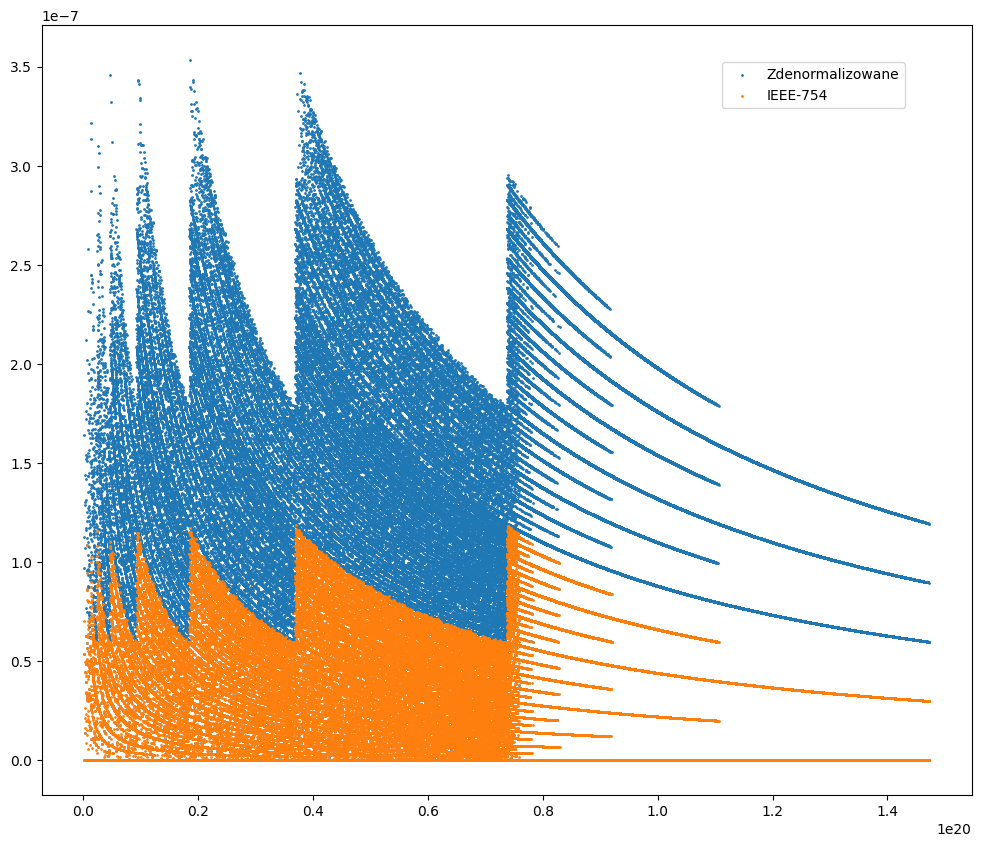
\includegraphics[height=0.4\textheight]{figures/add_relative.png}
	\caption{Błąd względny - dodawanie}
	\label{fig:add_relative}
\end{figure}

\begin{figure}[H]
	\centering
	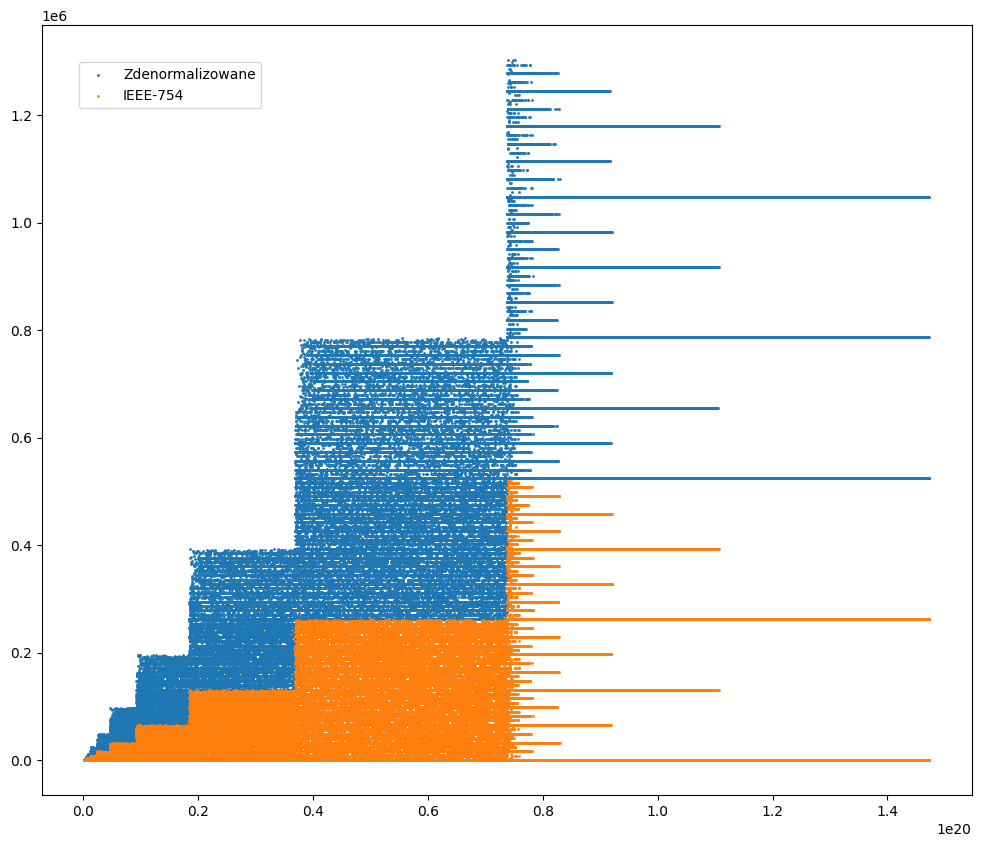
\includegraphics[height=0.4\textheight]{figures/add_ulp.png}
	\caption{Błąd bezwzględny - dodawanie}
	\label{fig:add_ulp}
\end{figure}


\begin{figure}[H]
	\centering
	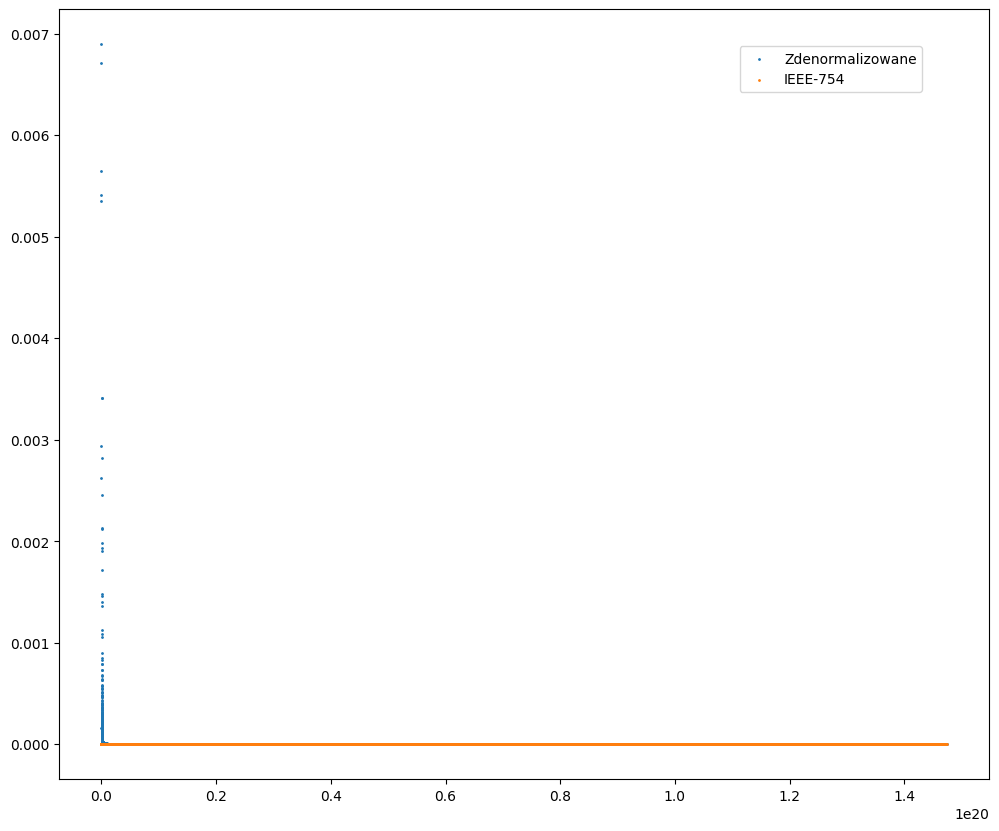
\includegraphics[height=0.4\textheight]{figures/sub_relative.png}
	\caption{Błąd względny - odejmowanie}
	\label{fig:sub_relative}
\end{figure}

\begin{figure}[H]
	\centering
	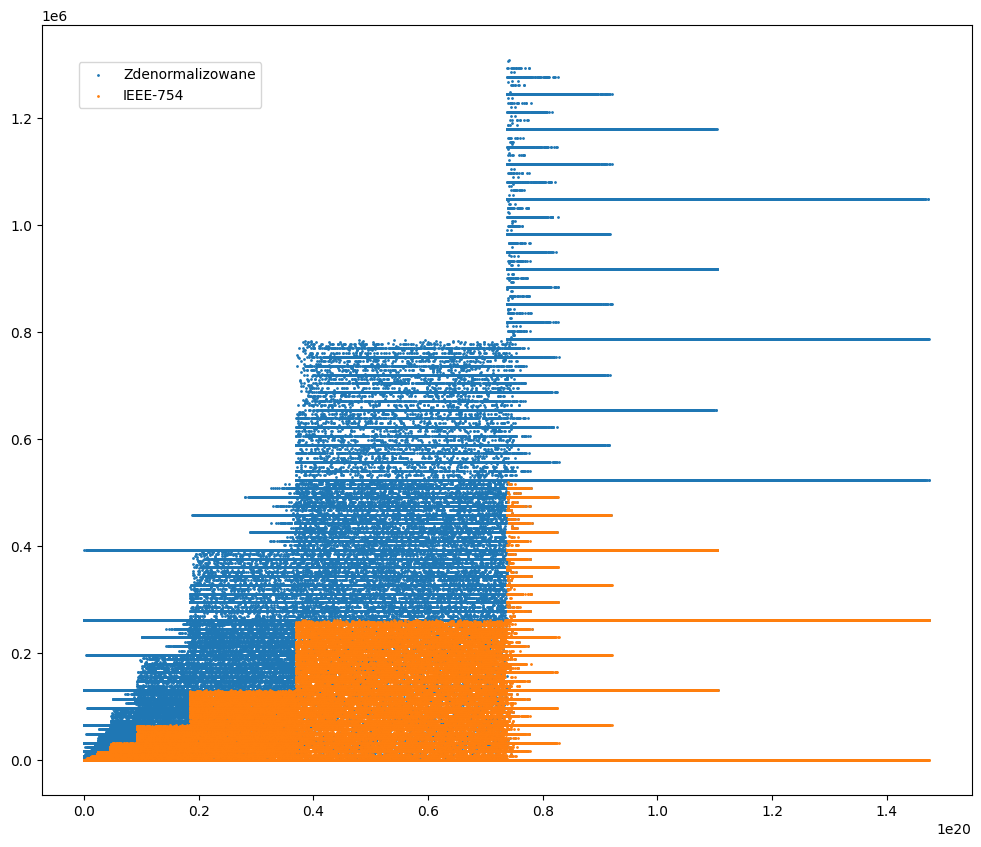
\includegraphics[height=0.4\textheight]{figures/sub_ulp.png}
	\caption{Błąd bezwzględny - odejmowanie}
	\label{fig:sub_ulp}
\end{figure}


\begin{figure}[H]
	\centering
	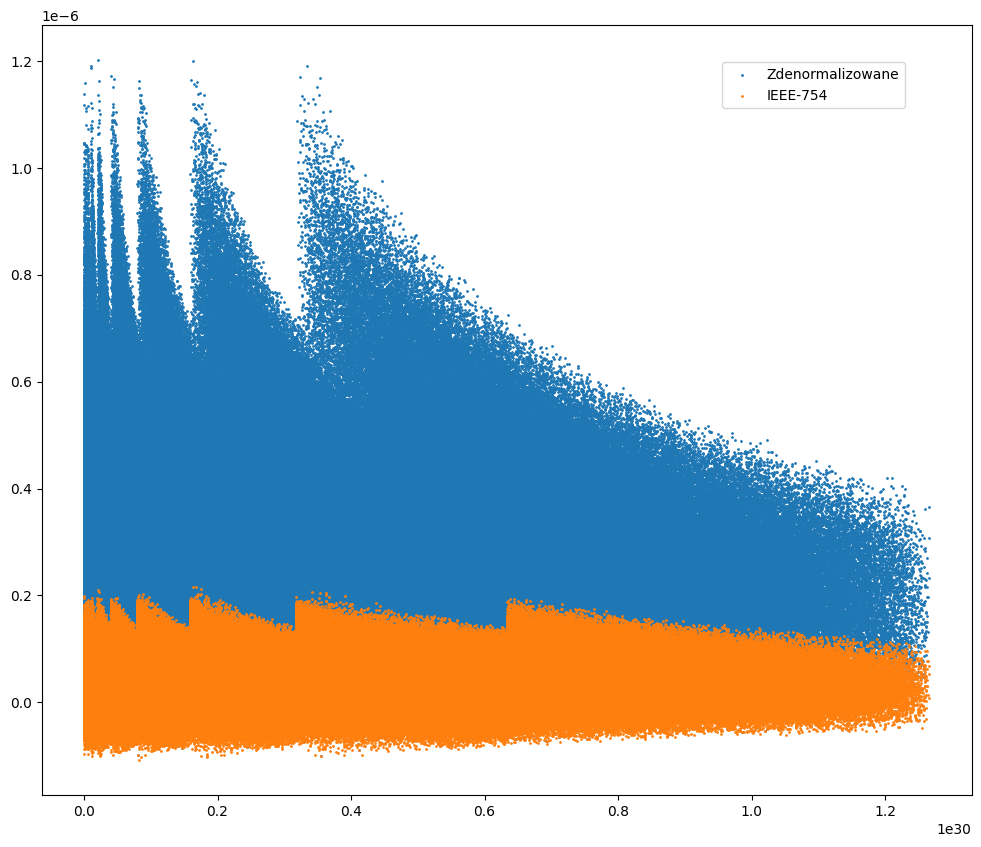
\includegraphics[height=0.4\textheight]{figures/mul_relative.png}
	\caption{Błąd względny - mnożenie}
	\label{fig:mul_relative}
\end{figure}

\begin{figure}[H]
	\centering
	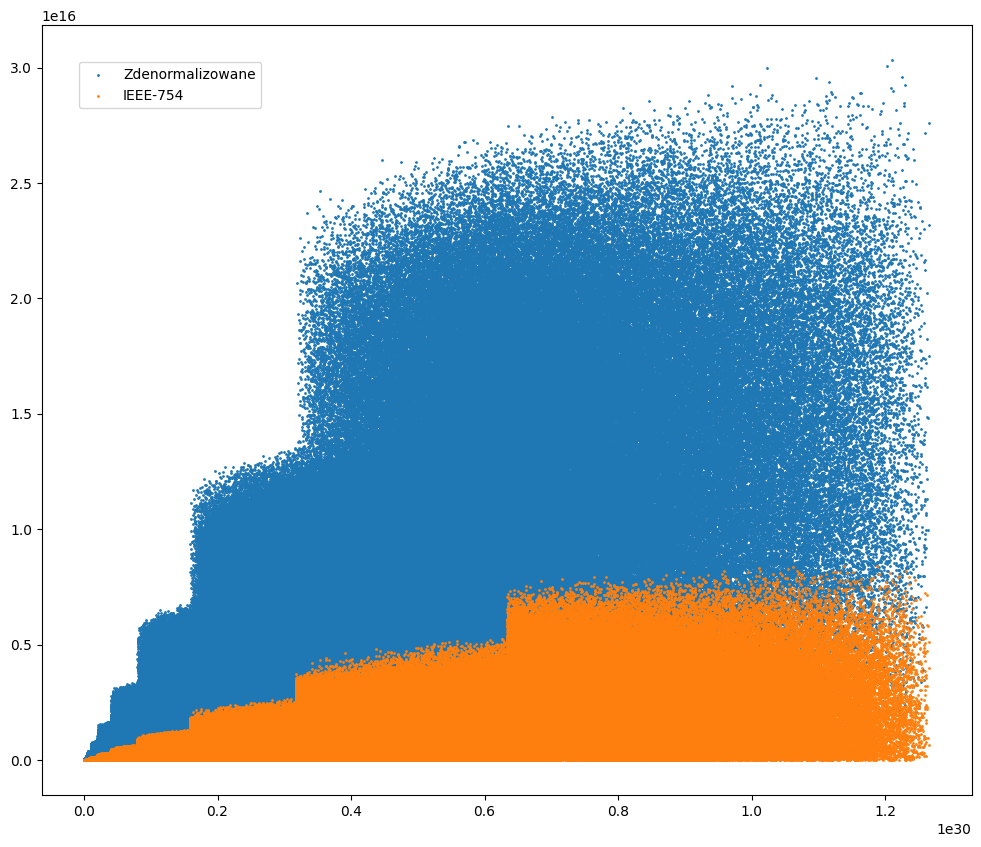
\includegraphics[height=0.4\textheight]{figures/mul_ulp.png}
	\caption{Błąd bezwzględny - mnożenie}
	\label{fig:mul_ulp}
\end{figure}


\section{Wnioski}
Podstawową i najbardziej zauważalną cechą jest wydzielenie się dwóch grup punktów przedstawiających wyniki dla liczb zdenormalizowanych i znormalizowanych.
W pomiarach widzimy różnicę w utracie dokładności jako wynik przesunięcia wszystkich bitów w prawo i pozbycia się ukrytego bitu w liczbach zdenormalizowanych.
Różnice w działaniu układów sprawiają, że implementacja dla liczb zdenormalizowanych jest prostsza, zużywa mniej komponentów, a przez to powinna zużywać mniej energii.

Poziome linie powstałe na wykresie są wynikiem stałej liczby bitów reprezentacji liczby.
Ponieważ zbiór liczb możliwych do przedstawienia w każdym z badanych zapisów jest skończony, to wyniki są zaokrąglane, a widoczne linie są tego efektem.
Mniej więcej w połowie wykresu widoczna jest granica, po której punkty układają się na wspomnianych liniach.
Granica jest wynikiem ograniczonej liczby bitów na część ułamkową.

Żeby zminimalizować straty w precyzji wyników, autorzy artykułu \cite{art:old} zaproponowali kolejne wersje układów.
Wprowadzają one większe zmiany niż odtworzone przez nas układy.
Są one zaprezentowane i opisane w artykule \cite{art:new} oraz prezentacji \cite{pdf:pres}.

% ponieważ podczas operacji odejmowania mantysy dążą do zera, to w ieee754 dwukrotnie większa ilość bitów (48) na wynik sprawia, że można wcześniej przesunięte bity "wrócić" podczas normalizacji, gdzie dla zdenormalizowanych nawet, gdyby te bity tam były, to nic by ich nie przesunęło bo nie ma normalizacji

\section{Kod źródłowy (dostępny pod \cite{url:github})}

\subsection{benches/adder.py}

\begin{lstlisting}
import struct
import ctypes
import subprocess
from statistics import mean, stdev
from random import uniform

subprocess.run(
    ["gcc", "-shared", "utils.c", "-o", "utils.so"])

utils = ctypes.CDLL("./utils.so")

py2float = utils.py2float
py2float.argtypes = [ctypes.c_float]
py2float.restype = ctypes.c_float
py2double = utils.py2double
py2double.argtypes = [ctypes.c_float]
py2double.restype = ctypes.c_double
add_floats = utils.add_floats
add_floats.argtypes = [ctypes.c_float, ctypes.c_float]
add_floats.restype = ctypes.c_float
add_doubles = utils.add_doubles
add_doubles.argtypes = [ctypes.c_double, ctypes.c_double]
add_doubles.restype = ctypes.c_double
add_true_doubles = utils.add_true_doubles
add_true_doubles.argtypes = [
    ctypes.c_double, ctypes.c_double]
add_true_doubles.restype = ctypes.c_double


def generate_random():
    return uniform(-73786971896791695000, 73786971896791695000)
    # return uniform(0, 73786971896791695000)


def double_to_hex(d):
    h = hex(struct.unpack("<Q", struct.pack("<d", d))[0])
    return h[2:].zfill(16)


def hex_to_double(h):
    return struct.unpack("!d", bytes.fromhex(h))[0]


def float_to_hex(f):
    h = hex(struct.unpack("<I", struct.pack("<f", f))[0])
    return h[2:].zfill(8)


def hex_to_float(h):
    return struct.unpack("!f", bytes.fromhex(h))[0]


def hex_to_bits(h):
    bits = bin(int(h, 16))[2:].zfill(32)
    return [int(b) for b in bits]


def bits_to_hex(bits):
    bits_bin = "".join(map(str, bits))
    return hex(int(bits_bin, 2))[2:].zfill(8)


def normalized_bits_to_denormalized_bits(bits):
    s, e, f = bits[0], bits[1:9], bits[9:]
    if any(e):
        e_bin = "".join(map(str, e))
        new_e_int = int(e_bin, 2) + 1
        new_e_bin = bin(new_e_int)[2:].zfill(8)
        e = [int(b) for b in new_e_bin]

        f = [1, *f][:-1]

    return [s, *e, *f]


def denormalized_bits_to_normalized_bits(bits):
    s, e, f = bits[0], bits[1:9], bits[9:]

    new_f = [0, *f]
    e_bin = "".join(map(str, e))
    new_e_int = int(e_bin, 2)
    for _ in range(23):
        if new_f[0] == 1:
            break

        new_f = [*new_f[1:], 0]
        new_e_int -= 1

    new_e_bin = bin(new_e_int)[2:].zfill(8)
    new_e = [int(b) for b in new_e_bin]

    return [s, *new_e, *new_f[1:]]


def float_to_denormalized_hex(f):
    return bits_to_hex(
        normalized_bits_to_denormalized_bits(
            hex_to_bits(float_to_hex(f)))
    )


def denormalized_hex_to_float(h):
    return hex_to_float(
        bits_to_hex(
            denormalized_bits_to_normalized_bits(hex_to_bits(h)))
    )


tb_fadd = """`timescale 1ps/1ps

`include "fadd_ieee754.v"

module tb_fadd_ieee754;

reg [31:0] a, b;
wire [31:0] out;

reg clk = 1'b1;

fadd_ieee754 uut(a, b, out);

always clk = #5 ~clk;

initial begin

##REPLACE_THIS##
    \$finish;
end

task test_case(
    input [31:0] a_in,
    input [31:0] b_in
); begin
    @(negedge clk) begin
        a = a_in;
        b = b_in;
    end
    @(posedge clk) begin
        \$display("%h", out);
    end
end
endtask

endmodule
"""

tb_fadd_denorm = tb_fadd.replace(
    "fadd_ieee754", "fadd_denorm")

NUMBER_OF_TESTS = 1000000


def main():
    double_result_list = []
    tb_fadd_tests = ""
    tb_fadd_denorm_tests = ""
    for _ in range(NUMBER_OF_TESTS):
        a, b = generate_random(), generate_random()
        a_float, b_float = py2float(a), py2float(b)

        a_hex_float, b_hex_float = 
            float_to_hex(a_float), float_to_hex(b_float)
        a_hex_denorm = float_to_denormalized_hex(a_float)
        b_hex_denorm = float_to_denormalized_hex(b_float)

        tb_fadd_tests +=
            f"\ttest_case(32'h{a_hex_float}, 32'h{b_hex_float});\n"
        tb_fadd_denorm_tests += (
            f"\ttest_case(32'h{a_hex_denorm}, 32'h{b_hex_denorm});\n"
        )
        double_result_list.append(add_doubles(a, b))

    with open("../src/fadd_ieee754/tb_fadd_ieee754_bench.v", "w") as f:
        f.write(tb_fadd.replace(
            "##REPLACE_THIS##", tb_fadd_tests))

    with open("../src/fadd_denorm/tb_fadd_denorm_bench.v", "w") as f:
        f.write(tb_fadd_denorm.replace(
            "##REPLACE_THIS##", tb_fadd_denorm_tests))

    print("files saved")

    subprocess.run(
        ["iverilog", "tb_fadd_ieee754_bench.v"],
        cwd="../src/fadd_ieee754/"
    )
    subprocess.run(
        ["iverilog", "tb_fadd_denorm_bench.v"],
        cwd="../src/fadd_denorm/"
    )

    results_float = (
        subprocess.run(
            ["./a.out"],
            stdout=subprocess.PIPE,
            cwd="../src/fadd_ieee754/",
        )
        .stdout.decode("utf8")
        .splitlines()
    )
    float_result_list = [
        hex_to_float(h) for h in results_float]
    results_denorm = (
        subprocess.run(
            ["./a.out"],
            stdout=subprocess.PIPE,
            cwd="../src/fadd_denorm/",
        )
        .stdout.decode("utf8")
        .splitlines()
    )
    denorm_result_list = [
        denormalized_hex_to_float(h) for h in results_denorm]

    denorm_errors = []
    float_errors = []
    print()
    fp_out = open("sub_out.csv", "w")
    # fp_out = open("add_out.csv", "w")
    for denorm, fnorm, double in zip(
        denorm_result_list,
        float_result_list,
        double_result_list,
    ):
        fp_out.write(f"{denorm},{fnorm},{double}\n")
        denorm_errors.append((double - denorm) / double)
        float_errors.append((double - fnorm) / double)

    fp_out.close()
    print(
        f"denormalized: {mean(denorm_errors)} ± {stdev(denorm_errors)}")
    print(
        f"float 754: {mean(float_errors)} ± {stdev(float_errors)}")

    subprocess.run(["rm", "./utils.so"])
    subprocess.run(
        [
            "rm",
            "../src/fadd_ieee754/a.out",
            "../src/fadd_ieee754/tb_fadd_ieee754_bench.v",
        ]
    )
    subprocess.run(
        ["rm", "../src/fadd_denorm/a.out",
            "../src/fadd_denorm/tb_fadd_denorm_bench.v"]
    )


if __name__ == "__main__":
    main()
\end{lstlisting}

\subsection{benches/graphs.py}

\begin{lstlisting}
import numpy as np
import matplotlib.pyplot as plt

# denormalized,ieee754,double
data_a = np.genfromtxt("add_out.csv", delimiter=",")
data_s = np.genfromtxt("sub_out.csv", delimiter=",")
data_m = np.genfromtxt("mult_out.csv", delimiter=",")

# relative difference

fig1 = plt.figure(figsize=(12, 10), dpi=100)

xa = data_a[:, 2]
ya1 = np.fromiter(
    ((r[2] - r[0]) / r[2] for r in data_a),
    dtype=float,
)
plt.scatter(xa, ya1, s=1)

ya2 = np.fromiter(
    ((r[2] - r[1]) / r[2] for r in data_a),
    dtype=float,
)
plt.scatter(xa, ya2, s=1)

plt.figlegend(
    ["Zdenormalizowane", "IEEE-754"],
    loc="upper right",
    bbox_to_anchor=(0.85, 0.85),
)
plt.savefig("add_relative.png", bbox_inches="tight")

fig2 = plt.figure(figsize=(12, 10), dpi=100)

xs = data_s[:, 2]
ys1 = np.fromiter(
    ((r[2] - r[0]) / r[2] for r in data_s),
    dtype=float,
)
plt.scatter(np.abs(xs), np.abs(ys1), s=1)

ys2 = np.fromiter(
    ((r[2] - r[1]) / r[2] for r in data_s),
    dtype=float,
)
plt.scatter(np.abs(xs), np.abs(ys2), s=1)

plt.figlegend(
    ["Zdenormalizowane", "IEEE-754"],
    loc="upper right",
    bbox_to_anchor=(0.85, 0.85)
)
plt.savefig("sub_relative.png", bbox_inches="tight")

fig3 = plt.figure(figsize=(12, 10), dpi=100)

xm = data_m[:, 2]
ym1 = np.fromiter(
    ((r[2] - r[0]) / r[2] for r in data_m),
    dtype=float,
)
plt.scatter(xm, ym1, s=1)

ym2 = np.fromiter(
    ((r[2] - r[1]) / r[2] for r in data_m),
    dtype=float,
)
plt.scatter(xm, ym2, s=1)

plt.figlegend(
    ["Zdenormalizowane", "IEEE-754"],
    loc="upper right",
    bbox_to_anchor=(0.85, 0.85)
)
plt.savefig("mul_relative.png", bbox_inches="tight")

# absolute (ulp) difference

fig4 = plt.figure(figsize=(12, 10), dpi=100)

xa = data_a[:, 2]
ya1 = np.fromiter(
    (abs(r[2] - r[0]) / 2 ** 24 for r in data_a),
    dtype=float,
)
plt.scatter(xa, ya1, s=1)

ya2 = np.fromiter(
    (abs(r[2] - r[1]) / 2 ** 24 for r in data_a),
    dtype=float,
)
plt.scatter(xa, ya2, s=1)

plt.figlegend(
    ["Zdenormalizowane", "IEEE-754"],
    loc="upper left",
    bbox_to_anchor=(0.15, 0.85)
)
plt.savefig("add_ulp.png", bbox_inches="tight")

fig5 = plt.figure(figsize=(12, 10), dpi=100)

xs = data_s[:, 2]
ys1 = np.fromiter(
    (abs(r[2] - r[0]) / 2 ** 24 for r in data_s),
    dtype=float,
)
plt.scatter(np.abs(xs), np.abs(ys1), s=1)

ys2 = np.fromiter(
    (abs(r[2] - r[1]) / 2 ** 24 for r in data_s),
    dtype=float)
plt.scatter(np.abs(xs), np.abs(ys2), s=1)

plt.figlegend(
    ["Zdenormalizowane", "IEEE-754"],
    loc="upper left",
    bbox_to_anchor=(0.15, 0.85)
)
plt.savefig("sub_ulp.png", bbox_inches="tight")

fig6 = plt.figure(figsize=(12, 10), dpi=100)

xm = data_m[:, 2]
ym1 = np.fromiter(
    (abs(r[2] - r[0]) / 2 ** 24 for r in data_m), 
    dtype=float,
)
plt.scatter(xm, ym1, s=1)

ym2 = np.fromiter(
    (abs(r[2] - r[1]) / 2 ** 24 for r in data_m),
    dtype=float,
)
plt.scatter(xm, ym2, s=1)

plt.figlegend(
    ["Zdenormalizowane", "IEEE-754"],
    loc="upper left",
    bbox_to_anchor=(0.15, 0.85)
)
plt.savefig("mul_ulp.png", bbox_inches="tight")

# plt.show()
\end{lstlisting}

\subsection{benches/mult.py}

\begin{lstlisting}
import struct
import ctypes
import subprocess
from statistics import mean, stdev
from random import uniform

subprocess.run(["gcc", "-shared", "utils.c", "-o", "utils.so"])

utils = ctypes.CDLL("./utils.so")

py2float = utils.py2float
py2float.argtypes = [ctypes.c_float]
py2float.restype = ctypes.c_float
py2double = utils.py2double
py2double.argtypes = [ctypes.c_float]
py2double.restype = ctypes.c_double
mult_floats = utils.mult_floats
mult_floats.argtypes = [ctypes.c_float, ctypes.c_float]
mult_floats.restype = ctypes.c_float
mult_doubles = utils.mult_doubles
mult_doubles.argtypes = [ctypes.c_double, ctypes.c_double]
mult_doubles.restype = ctypes.c_double
mult_doubles = utils.mult_true_doubles
mult_doubles.argtypes = [ctypes.c_double, ctypes.c_double]
mult_doubles.restype = ctypes.c_double


def generate_random():
    return uniform(0.000000000000000001, 1125899839733760)


def double_to_hex(d):
    h = hex(struct.unpack("<Q", struct.pack("<d", d))[0])
    return h[2:].zfill(16)


def hex_to_double(h):
    return struct.unpack("!d", bytes.fromhex(h))[0]


def float_to_hex(f):
    h = hex(struct.unpack("<I", struct.pack("<f", f))[0])
    return h[2:].zfill(8)


def hex_to_float(h):
    return struct.unpack("!f", bytes.fromhex(h))[0]


def hex_to_bits(h):
    bits = bin(int(h, 16))[2:].zfill(32)
    return [int(b) for b in bits]


def bits_to_hex(bits):
    bits_bin = "".join(map(str, bits))
    return hex(int(bits_bin, 2))[2:].zfill(8)


def normalized_bits_to_denormalized_bits(bits):
    s, e, f = bits[0], bits[1:9], bits[9:]
    if any(e):
        e_bin = "".join(map(str, e))
        new_e_int = int(e_bin, 2) + 1
        new_e_bin = bin(new_e_int)[2:].zfill(8)
        e = [int(b) for b in new_e_bin]

        f = [1, *f][:-1]

    return [s, *e, *f]


def denormalized_bits_to_normalized_bits(bits):
    s, e, f = bits[0], bits[1:9], bits[9:]

    new_f = [0, *f]
    e_bin = "".join(map(str, e))
    new_e_int = int(e_bin, 2)
    for _ in range(23):
        if new_e_int == 0:
            new_e_bin = bin(new_e_int)[2:].zfill(8)
            new_e = [int(b) for b in new_e_bin]
            return [s, *new_e, *new_f]
        if new_f[0] == 1:
            break

        new_f = [*new_f[1:], 0]
        new_e_int -= 1

    new_e_bin = bin(new_e_int)[2:].zfill(8)
    new_e = [int(b) for b in new_e_bin]

    return [s, *new_e, *new_f[1:]]


def float_to_denormalized_hex(f):
    return bits_to_hex(
        normalized_bits_to_denormalized_bits(
            hex_to_bits(float_to_hex(f)))
    )


def denormalized_hex_to_float(h):
    return hex_to_float(
        bits_to_hex(
            denormalized_bits_to_normalized_bits(hex_to_bits(h)))
    )

tb_fmult = """`timescale 1ps/1ps

`include "fmult_ieee754.v"

module tb_fmult_ieee754;

reg [31:0] a, b;
wire [31:0] out;

reg clk = 1'b1;

fmult_ieee754 uut(a, b, out);

always clk = #5 ~clk;

initial begin

##REPLACE_THIS##
    \$finish;
end

task test_case(
    input [31:0] a_in,
    input [31:0] b_in
); begin
    @(negedge clk) begin
        a = a_in;
        b = b_in;
    end
    @(posedge clk) begin
        \$display("%h", out);
    end
end
endtask

endmodule
"""

tb_fmult_denorm = tb_fmult.replace("fmult_ieee754", "fmult_denorm")

NUMBER_OF_TESTS = 1000


def main():
    double_result_list = []
    tb_fmult_tests = ""
    tb_fmult_denorm_tests = ""
    for _ in range(NUMBER_OF_TESTS):
        a, b = generate_random(), generate_random()
        a_float, b_float = py2float(a), py2float(b)

        a_hex_float, b_hex_float =
            float_to_hex(a_float), float_to_hex(b_float)
        a_hex_denorm = float_to_denormalized_hex(a_float)
        b_hex_denorm = float_to_denormalized_hex(b_float)

        tb_fmult_tests +=
            f"\ttest_case(32'h{a_hex_float}, 32'h{b_hex_float});\n"
        tb_fmult_denorm_tests += (
            f"\ttest_case(32'h{a_hex_denorm}, 32'h{b_hex_denorm});\n"
        )
        double_result_list.append(mult_doubles(a, b))

    with open("../src/fmult_ieee754/tb_fmult_ieee754_bench.v", "w") as f:
        f.write(
            tb_fmult.replace(
                "##REPLACE_THIS##",
                tb_fmult_tests
            )
        )

    with open("../src/fmult_denorm/tb_fmult_denorm_bench.v", "w") as f:
        f.write(
            tb_fmult_denorm.replace(
                "##REPLACE_THIS##",
                tb_fmult_denorm_tests
            )
        )

    subprocess.run(
        ["iverilog", "tb_fmult_ieee754_bench.v"],
        cwd="../src/fmult_ieee754/",
    )
    subprocess.run(
        ["iverilog",
        "tb_fmult_denorm_bench.v"],
        cwd="../src/fmult_denorm/",
    )

    results_float = (
        subprocess.run(
            ["./a.out"],
            stdout=subprocess.PIPE,
            cwd="../src/fmult_ieee754/",
        )
        .stdout.decode("utf8")
        .splitlines()
    )
    float_result_list = [hex_to_float(h) for h in results_float]
    results_denorm = (
        subprocess.run(
            ["./a.out"],
            stdout=subprocess.PIPE,
            cwd="../src/fmult_denorm/",
        )
        .stdout.decode("utf8")
        .splitlines()
    )
    denorm_result_list = [
        denormalized_hex_to_float(h) for h in results_denorm
    ]

    denorm_errors = []
    float_errors = []
    print()
    fp_out = open("mult_out.csv", "w")
    for denorm, fnorm, double in zip(
        denorm_result_list,
        float_result_list,
        double_result_list,
    ):
        fp_out.write(f"{denorm},{fnorm},{double}\n")
        denorm_errors.append((double - denorm) / double)
        float_errors.append((double - fnorm) / double)

    fp_out.close()
    print(f"denormalized: {mean(denorm_errors)} ± {stdev(denorm_errors)}")
    print(f"float 754: {mean(float_errors)} ± {stdev(float_errors)}")

    subprocess.run(["rm", "./utils.so"])
    subprocess.run(
        [
            "rm",
            "../src/fmult_ieee754/a.out",
            "../src/fmult_ieee754/tb_fmult_ieee754_bench.v",
        ]
    )
    subprocess.run(
        [
            "rm",
            "../src/fmult_denorm/a.out",
            "../src/fmult_denorm/tb_fmult_denorm_bench.v",
        ]
    )


if __name__ == "__main__":
    main()

\end{lstlisting}

\subsection{benches/utils.c}

\begin{lstlisting}
#include <stdio.h>

float py2float(float a) {
    // printf("a: %f\n", a);
    return a;
}

double py2double(float a) {
    // printf("a: %f, da: %lf\n", a, (double) a);
    return a;
}

float add_floats(float a, float b) {
    // printf("%f + %f = %f\n", a, b, a + b);
    return a + b;
}

double add_doubles(double a, double b) {
    // printf("%lf + %lf = %lf\n", a, b, a + b);
    return py2double(a) + py2double(b);
}

double add_true_doubles(double a, double b) {
    return a + b;
}

float mult_floats(float a, float b) {
    return a * b;
}

double mult_doubles(double a, double b) {
    return py2double(a) * py2double(b);
}

double mult_true_doubles(double a, double b) {
    return a * b;
}
\end{lstlisting}

\subsection{src/fadd\_denorm/fadd\_denorm.v}

\begin{lstlisting}
`include "sub8.v"
`include "mux.v"
`include "swap.v"
`include "r_shifter.v"
`include "u2_adder.v"

module fadd_denorm (
    input [31:0] a,
    input [31:0] b,
    output reg [31:0] out
);

    // setup a
    wire sign_a = a[31];
    wire [7:0] exponent_a = a[30:23];
    wire [22:0] fraction_a = a[22:0]; 

    // setup b
    wire sign_b = b[31];
    wire [7:0] exponent_b = b[30:23];
    wire [22:0] fraction_b = b[22:0];

    // exponent difference
    wire [8:0] exponent_diff;
    wire [7:0] exponent_diff_abs, exponent_larger;

    sub8 ED (exponent_a, exponent_b, exponent_diff);

    wire sign_d = exponent_diff[8];

    mux MUX (exponent_a, exponent_b, sign_d, exponent_larger);

    assign exponent_diff_abs = sign_d ? -exponent_diff : exponent_diff;

    // fraction calculation
    wire [23:0] fraction_larger, fraction_shifted,
                fraction_smaller, fraction_sum,
                fraction_sum_abs, fraction_preshift,
                fraction_out;

    swap SWAP (
        fraction_a,
        fraction_b,
        sign_d,
        fraction_larger,
        fraction_preshift
    );

    r_shifter SHRED (
        fraction_preshift,
        exponent_diff_abs,
        fraction_shifted
    );

    wire different_signs = sign_a ^ sign_b;

    // conditional invert
    assign fraction_smaller = different_signs 
                            ? ~fraction_shifted
                            : fraction_shifted;

    // U2 adder with different_signs as carry in
    wire ovf;
    u2_adder U2A (
        fraction_larger,
        fraction_smaller,
        different_signs,
        fraction_sum,
        ovf
    );

    // calculate abolute value of fraction_sum
    assign fraction_sum_abs = (fraction_sum[23] & different_signs)
                                ? -fraction_sum : fraction_sum;

    // shift right 1 bit
    r_shifter R1SHIFT (fraction_sum_abs, {7'b0, ovf}, fraction_out);

    wire [7:0] exponent_out = exponent_larger + ovf;

    // calculate sign
    wire sign_out = (sign_d ? sign_b : sign_a) ^ fraction_sum[23] ^ ovf;

    always @(*) begin
        out = {sign_out, exponent_out, fraction_out[22:0]};
    end

endmodule
\end{lstlisting}

\subsection{src/fadd\_denorm/mux.v}

\begin{lstlisting}
module mux (
    input [7:0] in0,
    input [7:0] in1,
    input select,
    output [7:0] out
);

    assign out = select ? in1 : in0;

endmodule
\end{lstlisting}

\subsection{src/fadd\_denorm/r\_shifter.v}

\begin{lstlisting}
module r_shifter (
    input [23:0] to_be_shifted,
    input [7:0] amount,
    output [23:0] shifted
);

    assign shifted = to_be_shifted >> amount;

endmodule
\end{lstlisting}

\subsection{src/fadd\_denorm/sub8.v}

\begin{lstlisting}
module sub8 (
    input [7:0] a,
    input [7:0] b,
    output [8:0] diff
);

    assign diff = a - b;

endmodule
\end{lstlisting}

\subsection{src/fadd\_denorm/swap.v}

\begin{lstlisting}
module swap (
    input [22:0] a,
    input [22:0] b,
    input select,
    output [23:0] swapped_a,
    output [23:0] swapped_b
);

    assign swapped_a = {1'b0, select ? b : a};
    assign swapped_b = {1'b0, select ? a : b};

endmodule
\end{lstlisting}

\subsection{src/fadd\_denorm/tb\_fadd\_denorm.v}

\begin{lstlisting}
`timescale 1ps/1ps

`include "fadd_denorm.v"

module tb_fadd_denorm;

reg [31:0] a, b;
wire [31:0] out;

reg clk = 1'b1;

fadd_denorm uut(a, b, out);

always clk = #5 ~clk;

initial begin

	\$dumpfile("fadd_denorm_out.vcd");
	\$dumpvars(0, tb_fadd_denorm);

    test_case(32'h0000_0000, 32'h0000_0000, 32'h0000_0000);
    test_case(32'h8000_0000, 32'h0000_0000, 32'h8000_0000);
    test_case(32'h3FC0_0000, 32'h0000_0000, 32'h3FC0_0000);
    test_case(32'h0000_0000, 32'h3FC0_0000, 32'h3FC0_0000);
    test_case(32'h8000_0000, 32'hBFC0_0000, 32'hBFC0_0000);
    test_case(32'hBFC0_0000, 32'h8000_0000, 32'hBFC0_0000);
    test_case(32'h7F7F_FFFF, 32'h0000_0000, 32'h7F7F_FFFF);
    test_case(32'h0000_0000, 32'h7F7F_FFFF, 32'h7F7F_FFFF);
    test_case(32'h7F7F_FFFF, 32'h8000_0000, 32'h7F7F_FFFF);
    test_case(32'h0000_0000, 32'hFF7F_FFFF, 32'hFF7F_FFFF);
    test_case(32'h3FC0_0000, 32'h7F7F_FFFF, 32'h7F7F_FFFF);
    test_case(32'h7F7F_FFFF, 32'h3FC0_0000, 32'h7F7F_FFFF);
    test_case(32'h7F7F_FFFF, 32'h7C7F_FFFF, 32'h7fbf_0001);
    test_case(32'h7C7F_FFFF, 32'h7F7F_FFFF, 32'h7fbf_0001); 
    test_case(32'hFF7F_FFFF, 32'hFC7F_FFFF, 32'hFfbf_0001);
    test_case(32'hFC7F_FFFF, 32'hFF7F_FFFF, 32'hFfbf_0001);
    test_case(32'h4A02_7533, 32'h4928_FA97, 32'h4a0c_b3d8);
    test_case(32'h4928_FA97, 32'h4A02_7533, 32'h4a0c_b3d8);
    test_case(32'h4928_FA97, 32'hCA02_7533, 32'h4a07_c972);
    
    
    \$finish;
end

task test_case(
    input [31:0] a_in,
    input [31:0] b_in,
    input [31:0] expected_out
); begin
    @(negedge clk) begin
        a = a_in;
        b = b_in;
    end
    @(posedge clk) begin
        if (expected_out == out)
            \$display("Success: %h + %h = %h", a_in, b_in, out);
        else
            \$display(
                "Error:  %h + %h = %h | %h",
                a_in,
                b_in,
                out,
                expected_out
            );
    end
end
endtask

endmodule
\end{lstlisting}

\subsection{src/fadd\_denorm/u2\_adder.v}

\begin{lstlisting}
module u2_adder (
    input [23:0] in_a,
    input [23:0] in_b,
    input carry_in,
    output [23:0] out_sum,
    output ovf
);

    wire extra;

    assign {extra, out_sum} =
        {in_a[23], in_a}
        + {in_b[23], in_b}
        + carry_in;
    assign ovf = extra ^ out_sum[23];

endmodule
\end{lstlisting}

\subsection{src/fadd\_ieee754/fadd\_ieee754.v}

\begin{lstlisting}
`include "sub8.v"
`include "mux.v"
`include "swap.v"
`include "r_shifter.v"
`include "u2_adder.v"

module fadd_ieee754 (
    input [31:0] a,
    input [31:0] b,
    output reg [31:0] out
);

    // setup a
    wire sign_a = a[31];
    wire [7:0] exponent_a = a[30:23];
    wire [23:0] fraction_a = |exponent_a ? {1'b1, a[22:0]} : 24'b0; 

    // setup b
    wire sign_b = b[31];
    wire [7:0] exponent_b = b[30:23];
    wire [23:0] fraction_b = |exponent_b ? {1'b1, b[22:0]} : 24'b0;

    // exponent difference
    wire [8:0] exponent_diff;
    wire [7:0] exponent_diff_abs, exponent_larger;

    sub8 ED (exponent_a, exponent_b, exponent_diff);

    wire sign_d = exponent_diff[8];

    mux MUX (
        exponent_a,
        exponent_b,
        sign_d,
        exponent_larger
        );

    assign exponent_diff_abs = sign_d ? -exponent_diff : exponent_diff;

    // fraction calculation
    wire [48:0] fraction_larger, fraction_shifted,
                fraction_smaller, fraction_sum,
                fraction_sum_abs, fraction_preshift,
                fraction_prenorm;

    swap SWAP (
        fraction_a,
        fraction_b,
        sign_d,
        fraction_larger,
        fraction_preshift
    );

    r_shifter SHRED (
        fraction_preshift, 
        exponent_diff_abs,
        fraction_shifted
    );

    wire different_signs = sign_a ^ sign_b;

    // conditional invert
    assign fraction_smaller = different_signs
                            ? ~fraction_shifted
                            : fraction_shifted;

    // U2 adder with different_signs as carry in
    wire ovf;
    u2_adder U2A (
        fraction_larger,
        fraction_smaller,
        different_signs,
        fraction_sum,
        ovf
    );

    // calculate abolute value of fraction_sum
    assign fraction_sum_abs = (fraction_sum[48] & different_signs)
                            ? -fraction_sum : fraction_sum;

    // shift right 1 bit
    r_shifter R1SHIFT (fraction_sum_abs, {7'b0, ovf}, fraction_prenorm);

    wire [7:0] exponent_prenorm = exponent_larger + ovf;

    // calculate sign
    wire sign_out = (sign_d ? sign_b : sign_a) ^ fraction_sum[48] ^ ovf;

    // normalise result
    integer index;
    reg [47:0] fraction_out;
    reg [7:0] exponent_out;

    always @(*) begin

        fraction_out = fraction_prenorm[47:0];
        exponent_out = exponent_prenorm;
        if (different_signs) begin
            for (index = 22; index >= 0; index--) begin
                if (fraction_out[47] == 0) begin
                    fraction_out = fraction_out << 1;
                    exponent_out = exponent_out - 1;
                end
            end
        end

        out = {sign_out, exponent_out, fraction_out[46:24]};
    end

endmodule
\end{lstlisting}

\subsection{src/fadd\_ieee754/mux.v}

\begin{lstlisting}
module mux (
    input [7:0] in0,
    input [7:0] in1,
    input select,
    output [7:0] out
);

    assign out = select ? in1 : in0;

endmodule
\end{lstlisting}

\subsection{src/fadd\_ieee754/r\_shifter.v}

\begin{lstlisting}
module r_shifter (
    input [48:0] to_be_shifted,
    input [7:0] amount,
    output [48:0] shifted
);

    assign shifted = to_be_shifted >> amount;

endmodule
\end{lstlisting}

\subsection{src/fadd\_ieee754/sub8.v}

\begin{lstlisting}
module sub8 (
    input [7:0] a,
    input [7:0] b,
    output [8:0] diff
);

    assign diff = a - b;

endmodule
\end{lstlisting}

\subsection{src/fadd\_ieee754/swap.v}

\begin{lstlisting}
module swap (
    input [23:0] a,
    input [23:0] b,
    input select,
    output [48:0] swapped_a,
    output [48:0] swapped_b
);

    assign swapped_a = {1'b0, select ? b : a, 24'b0};
    assign swapped_b = {1'b0, select ? a : b, 24'b0};

endmodule
\end{lstlisting}

\subsection{src/fadd\_ieee754/tb\_add\_ieee754.v}

\begin{lstlisting}
`timescale 1ps/1ps

`include "fadd_ieee754.v"

module tb_fadd_ieee754;

reg [31:0] a, b;
wire [31:0] out;

reg clk = 1'b1;

fadd_ieee754 uut(a, b, out);

always clk = #5 ~clk;

initial begin

	\$dumpfile("fadd_ieee754_out.vcd");
	\$dumpvars(0, tb_fadd_ieee754);

    test_case(32'h4A36_00CA, 32'hC93C_97A8, 32'h4A06_DAE0);
    test_case(32'h498A_D804, 32'hCA1E_F022, 32'hC9B3_0840);
    test_case(32'h4AA4_6873, 32'h49CD_A038, 32'h4AD7_D081);
    test_case(32'hC9D5_32B0, 32'h490C_91C1, 32'hC98E_E9D0);
    test_case(32'hC8DE_2B1B, 32'h4A47_E514, 32'h4A2C_1FB1);
    test_case(32'h4A74_30F1, 32'h499E_2E20, 32'h4AA1_A400);
    test_case(32'h4991_E4C7, 32'h4A03_8953, 32'h4A4C_7BB6);
    test_case(32'hCA9A_68CA, 32'h4989_3EA4, 32'hCA70_3242);
    test_case(32'h463F_D1E1, 32'h4904_179B, 32'h4907_16E3);
    test_case(32'h4A13_673A, 32'h486E_B87C, 32'h4A22_52C2);
    test_case(32'hCA0F_7140, 32'h4863_1EB8, 32'hCA01_3F54);
    test_case(32'hC92E_1F26, 32'h4A82_43DB, 32'h4A58_FFEC);
    test_case(32'hCA39_75F3, 32'hC9C7_7708, 32'hCA8E_98BC);
    \$finish;
end

task test_case(
    input [31:0] a_in,
    input [31:0] b_in,
    input [31:0] expected_out
); begin
    @(negedge clk) begin
        a = a_in;
        b = b_in;
    end
    @(posedge clk) begin
        if (expected_out == out)
            \$display("Success: %h + %h = %h", a_in, b_in, out);
        else
            \$display(
                "Error:  %h + %h = %h | %h",
                a_in,
                b_in,
                out,
                expected_out
            );
    end
end
endtask

endmodule
\end{lstlisting}

\subsection{src/fadd\_ieee754/u2\_adder.v}

\begin{lstlisting}
module u2_adder (
    input [48:0] in_a,
    input [48:0] in_b,
    input carry_in,
    output [48:0] out_sum,
    output ovf
);

    wire extra;

    assign {extra, out_sum} =
        {in_a[48], in_a}
        + {in_b[48], in_b}
        + carry_in;
    assign ovf = extra ^ out_sum[48];

endmodule
\end{lstlisting}

\subsection{src/fmult\_denorm/fmult\_denorm.v}

\begin{lstlisting}
module fmult_denorm
(
    input [31:0] a,
    input [31:0] b,
    output reg[31:0] out
);
    // Sign of a and b
    wire sign_a, sign_b;

    // Exponent of a and b
    wire [7:0] exponent_a, exponent_b;

    // Fraction parts of inputs a and b
    wire [22:0] fraction_a, fraction_b;
    
    // Variable assignment
    assign {sign_a, exponent_a, fraction_a} = a;
    assign {sign_b, exponent_b, fraction_b} = b;
    
    // Calculating sign
    wire sign_out = sign_a ^ sign_b;

    // Multiplier of 2 fraction
    wire [47:0] fraction_product = fraction_a * fraction_b;
    wire [22:0] fraction_out = fraction_product[46:24];
    
    // Calculating exponent
    wire [8:0] exponent_out = exponent_a + exponent_b - 8'd127 + 1'd1;

    always @(*) begin
        if (a == 32'd0 || b == 32'd0) begin
            // a or b is 0
            out = 32'd0;
        end else if (exponent_out[8] == 1) begin
            out = 32'd0;
        end else begin
            // normal result
            out = {sign_out, exponent_out[7:0], fraction_out};
        end
    end

endmodule
\end{lstlisting}

\subsection{src/fmult\_ieee754/fmult\_ieee754.v}

\begin{lstlisting}
module fmult_ieee754
(
    input [31:0] a,
    input [31:0] b,
    output reg[31:0] out
);

    // setup a
    wire sign_a = a[31];
    wire [7:0] exponent_a = a[30:23];
    wire [23:0] fraction_a = |exponent_a ? {1'b1, a[22:0]} : 24'b0; 

    // setup b
    wire sign_b = b[31];
    wire [7:0] exponent_b = b[30:23];
    wire [23:0] fraction_b = |exponent_b ? {1'b1, b[22:0]} : 24'b0;

    // Calculating fractions product with width is 2 * fraction width
    wire [47:0] fraction_product = fraction_a * fraction_b;

    // If product result was of form 1X.XXXX...
    wire norm = fraction_product[47];

    // Normalising fraction of the result
    wire [22:0] fraction_out = norm
        ? fraction_product[46:24] : fraction_product[45:23];

    // Calculating exponent of the result from adding two input
    // exponents, subtracting bias and adding norm bit
    wire [8:0] exponent_out = exponent_a + exponent_b - 8'd127 + norm; 

    // Calculating sign of the result
    wire sign_out = sign_a ^ sign_b;

    always @(*) begin
        if (a == 32'd0 || b == 32'd0) begin
            // a or b is 0
            out = 32'd0;
        end else if (exponent_out[8] == 1) begin
            out = 32'd0;
        end else begin
            // normal result
            out = {sign_out, exponent_out[7:0], fraction_out};
        end
    end

endmodule
\end{lstlisting}

\subsection{src/fmult\_ieee754/tb\_fmult\_ieee754.v}

\begin{lstlisting}
`timescale 1ps/1ps

`include "fmult_ieee754.v"

module tb_fmult_ieee754;

reg [31:0] a, b;
wire [31:0] out;

reg clk = 1'b1;

fmult_ieee754 uut(a, b, out);

always clk = #5 ~clk;

initial begin

	\$dumpfile("fmult_out.vcd");
	\$dumpvars(0, tb_fmult_ieee754);

    test_case(32'h4234_851F, 32'h427C_851F, 32'h4532_10E9);
    test_case(32'h0200_0000, 32'h0200_0000, 32'h0000_0000);
    test_case(32'hC152_6666, 32'hC240_A3D7, 32'h441E_5374);
    test_case(32'h4049_999A, 32'hC166_3D71, 32'hC235_5062);
    test_case(32'h3ACA_62C1, 32'h3ACA_62C1, 32'h361F_FFFF);
    test_case(32'h4580_0000, 32'h4580_0000, 32'h4B80_0000);
    test_case(32'h0000_0000, 32'h0000_0000, 32'h0000_0000);
    test_case(32'hC152_6666, 32'h0000_0000, 32'h0000_0000);
    test_case(32'h7F80_0000, 32'h7F80_0000, 32'h7F80_0000);
    test_case(32'h7F80_0000, 32'hFF80_0000, 32'hFF80_0000);
    test_case(32'hFF80_0000, 32'h7F80_0000, 32'hFF80_0000);
    test_case(32'hFF80_0000, 32'hFF80_0000, 32'h7F80_0000);
    test_case(32'h7F80_0000, 32'h7F80_000D, 32'h7FC0_0000);

    \$finish;
end

task test_case(
    input [31:0] a_in,
    input [31:0] b_in,
    input [31:0] expected_out
); begin
    @(negedge clk) begin
        a = a_in;
        b = b_in;
    end
    @(posedge clk) begin
        if (expected_out == out)
            \$display("Success: %h + %h = %h", a_in, b_in, out);
        else
            \$display(
                "Error:  %h + %h = %h | %h",
                a_in,
                b_in,
                out,
                expected_out
            );
    end
end
endtask

endmodule
\end{lstlisting}


\newpage
\phantomsection
\addcontentsline{toc}{section}{Literatura}
\bibliography{bibliography}
\bibliographystyle{plabbrv}


\end{document}
